%        File: homework.tex
%     Created: 六 5月 26 09:00 下午 2018 C
% Last Change: 六 5月 26 09:00 下午 2018 C
%
\documentclass[UTF8,noindent]{ctexart}
\usepackage[a4paper,left=2.0cm,right=2.0cm,top=2.0cm,bottom=2.0cm]{geometry}
\usepackage{hyperref}
\usepackage{array}
\usepackage{url}
\usepackage{graphicx}
\usepackage{amsmath}
\usepackage{amssymb}
\usepackage{enumitem}
\usepackage{tikz}
\usepackage{forest}
\usepackage{float}
\usepackage{pgf}
\usetikzlibrary{graphs}
\usetikzlibrary{arrows,automata}
\usepackage{listings}
\usepackage{xcolor}
\lstset{language = c,numbers=left, keywordstyle= \color{ blue!70 },commentstyle=\color{red!50!green!50!blue!50}, frame=shadowbox, rulesepcolor= \color{ red!20!green!20!blue!20 } 
} 
\usetikzlibrary{graphs}
\title{$Chapter\ 6-HW01$}
\author{$2015K8009929049$\ 冯吕}
\date{\today}
\begin{document}
\maketitle
\zihao{5}
\CJKfamily{zhsong}
$6.1.2$解:
$a+a+(a+a+a+(a+a+a+a))$对应的$DAG$如下图所示:
\begin{center}
  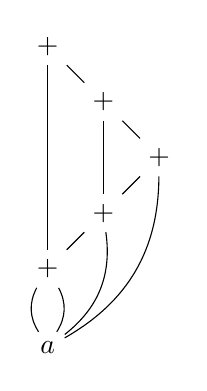
\begin{tikzpicture}
	\node (A)  {$+$};
	\node (B) [below right of = A] {$+$};
	\node (D) [below right of = B] {$+$};
	\node  (C) [below left of = D] {$+$};
	\node  (E) [below left of = C] {$+$};
	\node (F) [below of = E] {$a$};

  \path (A) edge  (B);
  \path (A) edge (E);
  \path (B) edge (C);
  \path (B) edge (D);
  \path (D) edge (C);
  \path (C) edge (E);
  \path (E) edge [bend left] (F);
  \path (C) edge [bend left] (F);
  \path (D) edge [bend left] (F);
  \path (E) edge [bend right] (F);

  \end{tikzpicture}
\end{center}
值编码如下:
\begin{center}
  \begin{tabular}{|p{2cm}<{\centering}|p{2cm}<{\centering}|p{2cm}<{\centering}|p{2cm}<{\centering}|}
	\hline
	$1$ & $id$ & $a$ &\\
	\hline
	$2$ & $+$ & $1$ & $1$\\
	\hline
	$3$ & $+$ & $2$ & $1$\\
	\hline
	$4$ & $+$ & $3$ &$1$ \\
	\hline
	$5$ & $+$ & $3$ & $4$ \\
	\hline
	$6$ & $+$ & $2$ & $5$\\
	\hline
  \end{tabular}
\end{center}

$6.2.1$解:
\begin{itemize}
  \item $(1)$抽象语法树:
	\begin{center}
	  \begin{forest}
		for tree = {math content}
		[+
		  [a]
		  [-
			[+
			  [b]
			  [c]
			]
		  ]
		]
	  \end{forest}
	\end{center}
  \item $(2)$ 四元式序列:
	\begin{center}
  \begin{tabular}{|p{2cm}<{\centering}|p{2cm}<{\centering}|p{2cm}<{\centering}|p{2cm}<{\centering}|p{2cm}<{\centering}|}
	\hline
	& $op$ & $arg1$ & $arg2$ & $result$\\
	\hline
	$0$ & $+$ & $b$ & $c$ & $t_1$\\
	\hline
	$1$ & $minus$ & $t_1$ & & $t_2$\\
	\hline
	$2$ & $+$ & $a$ & $t_2$ & $t_3$\\
	\hline
  \end{tabular}
	\end{center}

  \item $(3)$三元式序列:
	\begin{center}
  \begin{tabular}{|p{2cm}<{\centering}|p{2cm}<{\centering}|p{2cm}<{\centering}|p{2cm}<{\centering}|}
	\hline
	& $op$ & $arg1$ & $arg2$\\
	\hline 
	$0$ & $+$ & $b$ & $c$\\
	\hline
	$1$ & $minus$ & $(0)$ &\\
	\hline
	$2$ & $+$ & $a$ & $(1)$\\
	\hline
  \end{tabular}
	\end{center}
  \item $(4)$间接三元式序列:
	\begin{center}
  \begin{tabular}{|p{2cm}<{\centering}|p{2cm}<{\centering}|p{2cm}<{\centering}|p{2cm}<{\centering}|}
	\hline
	& $op$ & $arg1$ & $arg2$\\
	\hline 
	$(0)$ & $+$ & $b$ & $c$\\
	\hline
	$(1)$ & $minus$ & $(0)$ &\\
	\hline
	$(2)$ & $+$ & $a$ & $(1)$\\
	\hline
  \end{tabular}
  \quad
  \begin{tabular}{|p{2cm}<{\centering}|p{2cm}<{\centering}|}
	\hline
	& $instruction$\\
	\hline
	$0$ & $(0)$\\
	\hline
	$1$ & $(1)$\\
	\hline
	$2$ & $(2)$\\
	\hline
  \end{tabular}
	\end{center}
\end{itemize}
\end{document}
